\documentclass[letterpaper, 12pt]{article} % Feel free to change this
\usepackage{graphicx}
\usepackage{amsmath}
\usepackage{caption}
\usepackage[margin=1in]{geometry}

\begin{document}
\begin{titlepage}
	\centering
	
\includegraphics[width=0.2\textwidth]{Images/Duke_logo.png}\par\vspace{1cm}
	{\scshape\LARGE Duke University \par}
	\vspace{1cm}
	{\scshape\Large ECE 559: Advanced Digital Systems \par}
	\vspace{1.5cm}
	{\huge\bfseries Turbo Coder Internal Interleaver \par}
	\vspace{2cm}
   {By submitting this \LaTeX{} document, I affirm that it complies with the Duke Community Standard and the guidelines set forth for this assignment.\par}
   \vspace{1cm}
	{\Large Vinith Sharma, Yao Yuang, Cheng Lyu}
	\vfill
% Bottom of the page
	{\large Fall 2019\par}
\end{titlepage}


\newpage
\section{3GPP LTE Advanced Wireless System}
    \subsection{Introduction}
        The next advancement on wireless communication was proposed by the 3rd Generation Partnership Program (3GPP). Formally a candidate 4G to ITU-T in 2009, it was standardized in March of 2011.
        The biggest benefit of LTE Advanced is the ability to take advantage of avdanced topology networks. The usage of optimized heterogeneous networks and utilizing macrocells with low power nodes such as pico and femto cells create a much better network compared to macrocells (wide area high power base stations that covers a large radius). LTE Advanced also introduces multicarrier so we can utilize wider bandwidth, up to 100 MHz, which will support high data rates.

        Our focus this semester lied on the coding, multiplexing and mapping to physical channels for E-UTRA section of the LTE Advanced specification as seen in 3GPP TS 36.212 V10.5.0. The sub-systems extracted from this document that our class worked on is as follows:
        \begin{itemize}
            \item Code block segmentation and CRC
            \item Convolutional encoder
            \item Turbo-code constituent encoder
            \item Turbo-code interleaver
            \item Sub-block interleaver and multiplexer
        \end{itemize}
    \subsection{Internal Interleaver}
        Our group was responsible for the turbo coder internal interleaver. The purpose of this sub-system is to block interleave the data, frame quality indicator (CRC), and the reserve bits input to the turbo encoder. This interleaving happens through a index generator function defined in section 5.1.3.2.3 of the document. First we define an index generator function that selects the certain index of output bits from a certain input bit index. We will call this $\Pi(i)$:
        $$\Pi(i) = (f_1\cdot i + f_2\cdot i^2 )\mod K$$
        where $f_1$, $f_2$ are defined in Table 5.1.3-3 in the 3GPP document. These values depend on the block size $K$. In our case, $K$ could only be two different sizes 1056 and 6144. This leads us to the following values for $f_1$ and $f_2$:
        \renewcommand\arraystretch{1.2}
        \begin{center}
            \begin{tabular}{|c|c|c|}
            \hline
                $K$ & $f_1$ & $f_2$  \\ \hline
                1056 & 17 & 66 \\ \hline
                6144 & 263 & 480 \\ \hline
            \end{tabular}
        \end{center}
        Using these values, we can generate the output bits using the following function:
        $$c'_i = c_{\Pi(i)} \quad\forall i \in \{0, 1, 2, ..., K\}$$
        where $c_i$ is the $i^{th}$ bit of the input sequence and $c'_i$ is the $i^{th}$ bit of the output sequence defined by the function $\Pi(i)$.

        This sub-module is part of the larger sub-system, turbo-code constituent encoder. The turbo encoder's purpose is to encode the incoming data, CRC, and the two reserved bits. During encoding, the output tail sequence is also added. The encoder generates the output based on the code rate. In our case, the code rate was 1/3. It uses two systematic, recursive, convolutional encoders connected in parallel with an interleaver for the second encoder. The two recursive convolutional codes are called the constituents codes of the turbo code. Since there is delay after the interleaver processes the data, the second encoder must account for this delay of the incoming data sequence.
\section{Description of the design}
    2.  Description of the design, including:
        (mostly yao)
         o  interfaces to other functions in the encoder stack
        (mostly yao)
         o  identification of the data path through the function and
		    how the data path is controlled by FSMs, shown using a
			block diagram of the design as implemented.
         o  for data path and associated combinational logic (not FSMs), include
            the RTL view from Quartus, with a brief prose description;  this can
            be used to describe the block diagram mentioned in the
			previous bullet

		(mostly yao)
         o  FSM designs, with pictorial description (state transition diagrams)
            and text, clearly indicating what each state
            represents, how inputs determine the next state and Moore and Mealy
            outputs for each state, and also an indication of how the FSM is
            related to data flow through the function
\section{Static timing analysis}
(mostly cheng)
    3.  Static timing analysis
		 o  from the static timing analysis results, identify (a) worst-case slack
		 	against setup violations;  (b) maximum frequency at which the design
			can be clocked;  (c) the critical path corresponding to the worst-case
			slack.
		 o	based on the max frequency, comment on the max throughput that can
		 	be sustained by the function given the current design
\section{Simulation results}
(mostly yao)
	4.  Simulation results
         o  what was simulated, what were the test conditions, what is the
            significance of the test in the context of the subsystem function
         o  show on the plots of the results, by clear annotation on the plots,
            and in a prose discription, what the simulation results indicate with
            respect to operation and performance of the subsystem

\section{Hardware test results}
Initial concerns about the simulation was the size of the blocks and the number of bits we have to deal with. Trying to check every bit in a block of size 6144 would take an unnecessary amount of time. Thus, Vinith wrote a python script that simulated this sub-module. Listing \ref{simfunc} is a python function that takes in two parameters \texttt{input\_num}, the input sequence represented as a bitstring, and \texttt{flag\_6144}, a one bit number that represents the size of the block. Writing 6144 bits would also take a tremendous amount of time and any sort of recurring pattern in the input will be present in the output, thus Listing \ref{rng} is another function that generates a random bitstring of size specified inside the \texttt{range()} function in the \texttt{for} loop.
The initial hardware testing was done using a \texttt{reg} with a constant value and passing all the bits in block side $K$ into our interleaving module. The clock did not matter for this because everything was done instantaneously as this test was essentially rewiring the wires based on the input values. We then took the bottom 10 bits of the output sequence and displayed it using the LEDs in the FPGA. After verifying that the output sequence matched, we moved on to the next part in hardware testing: simulating an incoming bit sequence.
\newline
The test above did not really tell us how it would be used in real life, thus we had to incorporate a mechanism that simulated an incoming n-bit wide sequence. We skipped the bit-serial implementation and tested a byte-serial implementation. We created a byte-shift register that is 6144 bit wide. Since we did not have the code segmentation unit block, we used a read-only memory to hold the input sequence. Using a counter up to $\frac{6144}{8} = 768$, we took the values out of the ROM and fed it into the shift register. After 768 cycles, we latched the value onto a buffer register and fed it into our interleaving module. The output value was once again latched onto another register and displayed using the LEDs and 7-segment displayed found on the FPGA. This test was done with a 50 Hz clock so we could visibly see the counter incrementing and the values from ROM being shifted into the shift register. The first and last three bytes of \texttt{mif} file that was loaded onto the ROM is as follows:
\begin{multicols}{2}
\begin{enumerate}
\setcounter{enumi}{-1}
    \item $11110111_2$ $\longrightarrow$ F$7_{16}$
    \item $00111100_2$ $\longrightarrow$ 3C$_{16}$
    \item $11000110_2$ $\longrightarrow$ C$6_{16}$
\setcounter{enumi}{764}
    \item $11111000_2$ $\longrightarrow$ F$8_{16}$
    \item $01111110_2$ $\longrightarrow$ 7E$_{16}$
    \item $00111011_2$ $\longrightarrow$ 3B$_{16}$
\end{enumerate}
\end{multicols}
where the list index is the address in memory. Since the value is shifted right, we had to invert the original input and slice it into 8 bits.
This was verified as seen in Figure \ref{fpga1} and Figure \ref{fpga2}. Of the five seven segment displays, the left three are used to show the counter as it increments from 000 to 2FF in base 16. The right two displays are used to show the output byte as we shift it into the byte-shift register. We then took the 8 LSB and displayed it using the LEDs present in the FPGA. According to the output from the python script, the least significant byte for that input is: 10111111. This is also verified from Figure \ref{fpga2} as the right most 8 LEDs are correctly turned on in that order.
Since the logic analyzer did not work, we were unable to test extensively using the display.

\begin{figure}
\centering
\begin{subfigure}{.5\textwidth}
  \centering
  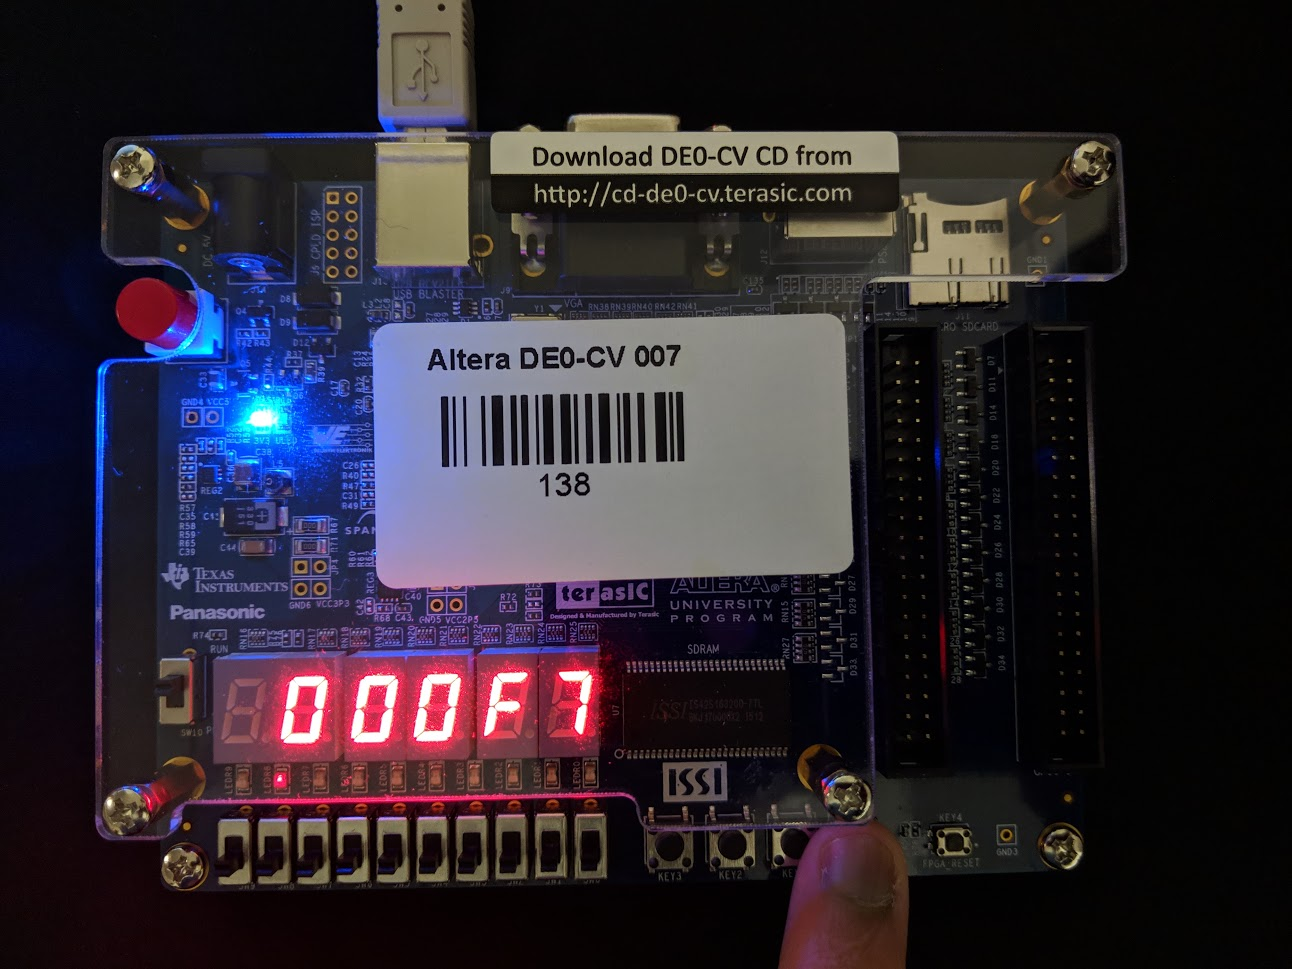
\includegraphics[width=0.99\linewidth]{files/add_zero}
  \caption{Initial state}
  \label{fpga1}
\end{subfigure}%
\begin{subfigure}{.5\textwidth}
  \centering
  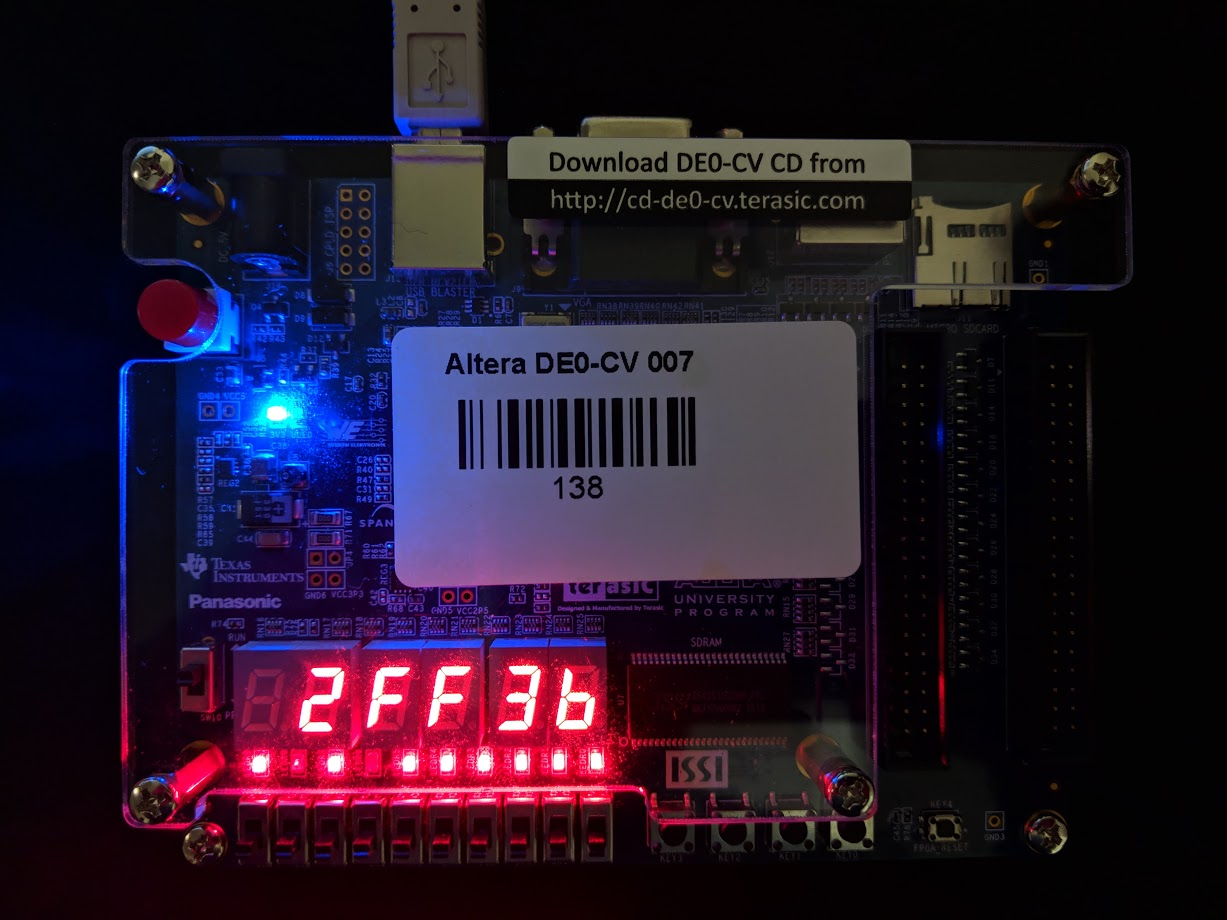
\includegraphics[width=0.99\linewidth]{files/add_2ff}
  \caption{Final state with LEDs}
  \label{fpga2}
\end{subfigure}
\caption{The initial and final state of the simulation as the data from ROM is put into the shift register. The LEDs represent the 8 output LSB bits.}
\label{fig:test}
\end{figure}

\newpage
\section*{Appendix}
\lstinputlisting[label = simfunc, language=Python, firstline=6, lastline=16, caption = {[Simulator Function]The function that simulates the interleaver.}, frame = lines]{files/test.py}

\lstinputlisting[label = rng, language=Python, firstline=21, lastline=26, frame = lines, caption = {[Random Block Generator]The function that generates a random block with uniform random bits as well as input last bit.}]{files/test.py}


\end{document}
